\documentclass[
letterpaper,
12pt,
oneside,
onecolumn, %twocolumn para dos columnas
article
]{memoir}

\usepackage[spanish,es-nodecimaldot]{babel}
\usepackage[utf8]{inputenc}
\usepackage[T1]{fontenc}
\usepackage{tgtermes} % La fuente a usar, si no compila quitar esta línea

\usepackage{macros}

\usepackage[final]{microtype}
\usepackage{graphicx} % Para incluir figuras
\usepackage{lipsum}

\usepackage{hyperref}

%%%%%%%%%%%%%%%%%%%%%%%%%%%%%%%%%%%%%%%%%%%%%%%%%%%%%%%%%
%% Aquí se modifica el formato, no modificar
%%%%%%%%%%%%%%%%%%%%%%%%%%%%%%%%%%%%%%%%%%%%%%%%%%%%%%%%%

\setlrmarginsandblock{0.15\paperwidth}{*}{1} % Para onecolumn
\setulmarginsandblock{1.5in}{2in}{1}  % Márgenes superior e inferior
\checkandfixthelayout

\addto{\captionsspanish}{%
  \renewcommand{\bibname}{\Large Referencias}
}

\counterwithout{section}{chapter}
\counterwithout{figure}{chapter}

\makeatletter
\def\@maketitle{%
  \newpage
  \null
  \vskip 2em%
  \let \footnote \thanks
  \begin{center}
    {\LARGE \textsc \@title \par}%
    \vskip 0.5em%
    {\large Probabilidad \textsc{ii} \par}
    \vskip 0.5em%
    {\large
      \lineskip .5em%
      \begin{tabular}[t]{c}%
        \@author
      \end{tabular}\par}%
    \vskip 1em%
    %{\large \@date}%
  \end{center}
  \par
  \vskip 1.5em}
\makeatother

\makepagestyle{plain}
\makeevenfoot{plain}{\thepage}{}{}
\makeoddfoot{plain}{}{}{\thepage}
\makeevenhead{plain}{}{}{}
\makeoddhead{plain}{}{}{}

%%%%%%%%%%%%%%%%%%%%%%%%%%%%%%%%%%%%%%%%%%%%%%%%%%%%%%%%%
%% Modificar desde aquí
%%%%%%%%%%%%%%%%%%%%%%%%%%%%%%%%%%%%%%%%%%%%%%%%%%%%%%%%%

\title{Tarea $\# \cdot$} % Cambiar título
\author{Nombre del alumno} % Su nombre

\begin{document}
\thispagestyle{empty}
\maketitle

\epigraph{Aquí pueden poner alguna cita para que su tarea parezca inspirada por}{Su autor preferido}

\Problema Aquí va el primer problema de la tarea.

\LaSolucion Aquí vamos a poner nuestra solución, donde tendremos $x = y$ y 
\[
\PP(X = x) = \PP(X = y),
\]
además de
\begin{align*}
    \PP(X \in (x -\varepsilon, x + \varepsilon)) & = \int \1_{(x -\varepsilon, x + \varepsilon)}(t)  \PP(dt) \\
    & = \int \1_{(y -\varepsilon, y + \varepsilon)}(t)  \PP(dt) \\
    & = \PP(X \in (y -\varepsilon, y + \varepsilon)).
\end{align*}

\Problema Aquí va el segundo problema para el que hicimos dos soluciones.

\UnaSolucion Cualquier cosa.

\UnaSolucion Aquí hasta dibujito hicimos y está en la figura \ref{galton watson}.

\begin{figure}[ht]
    \centering
    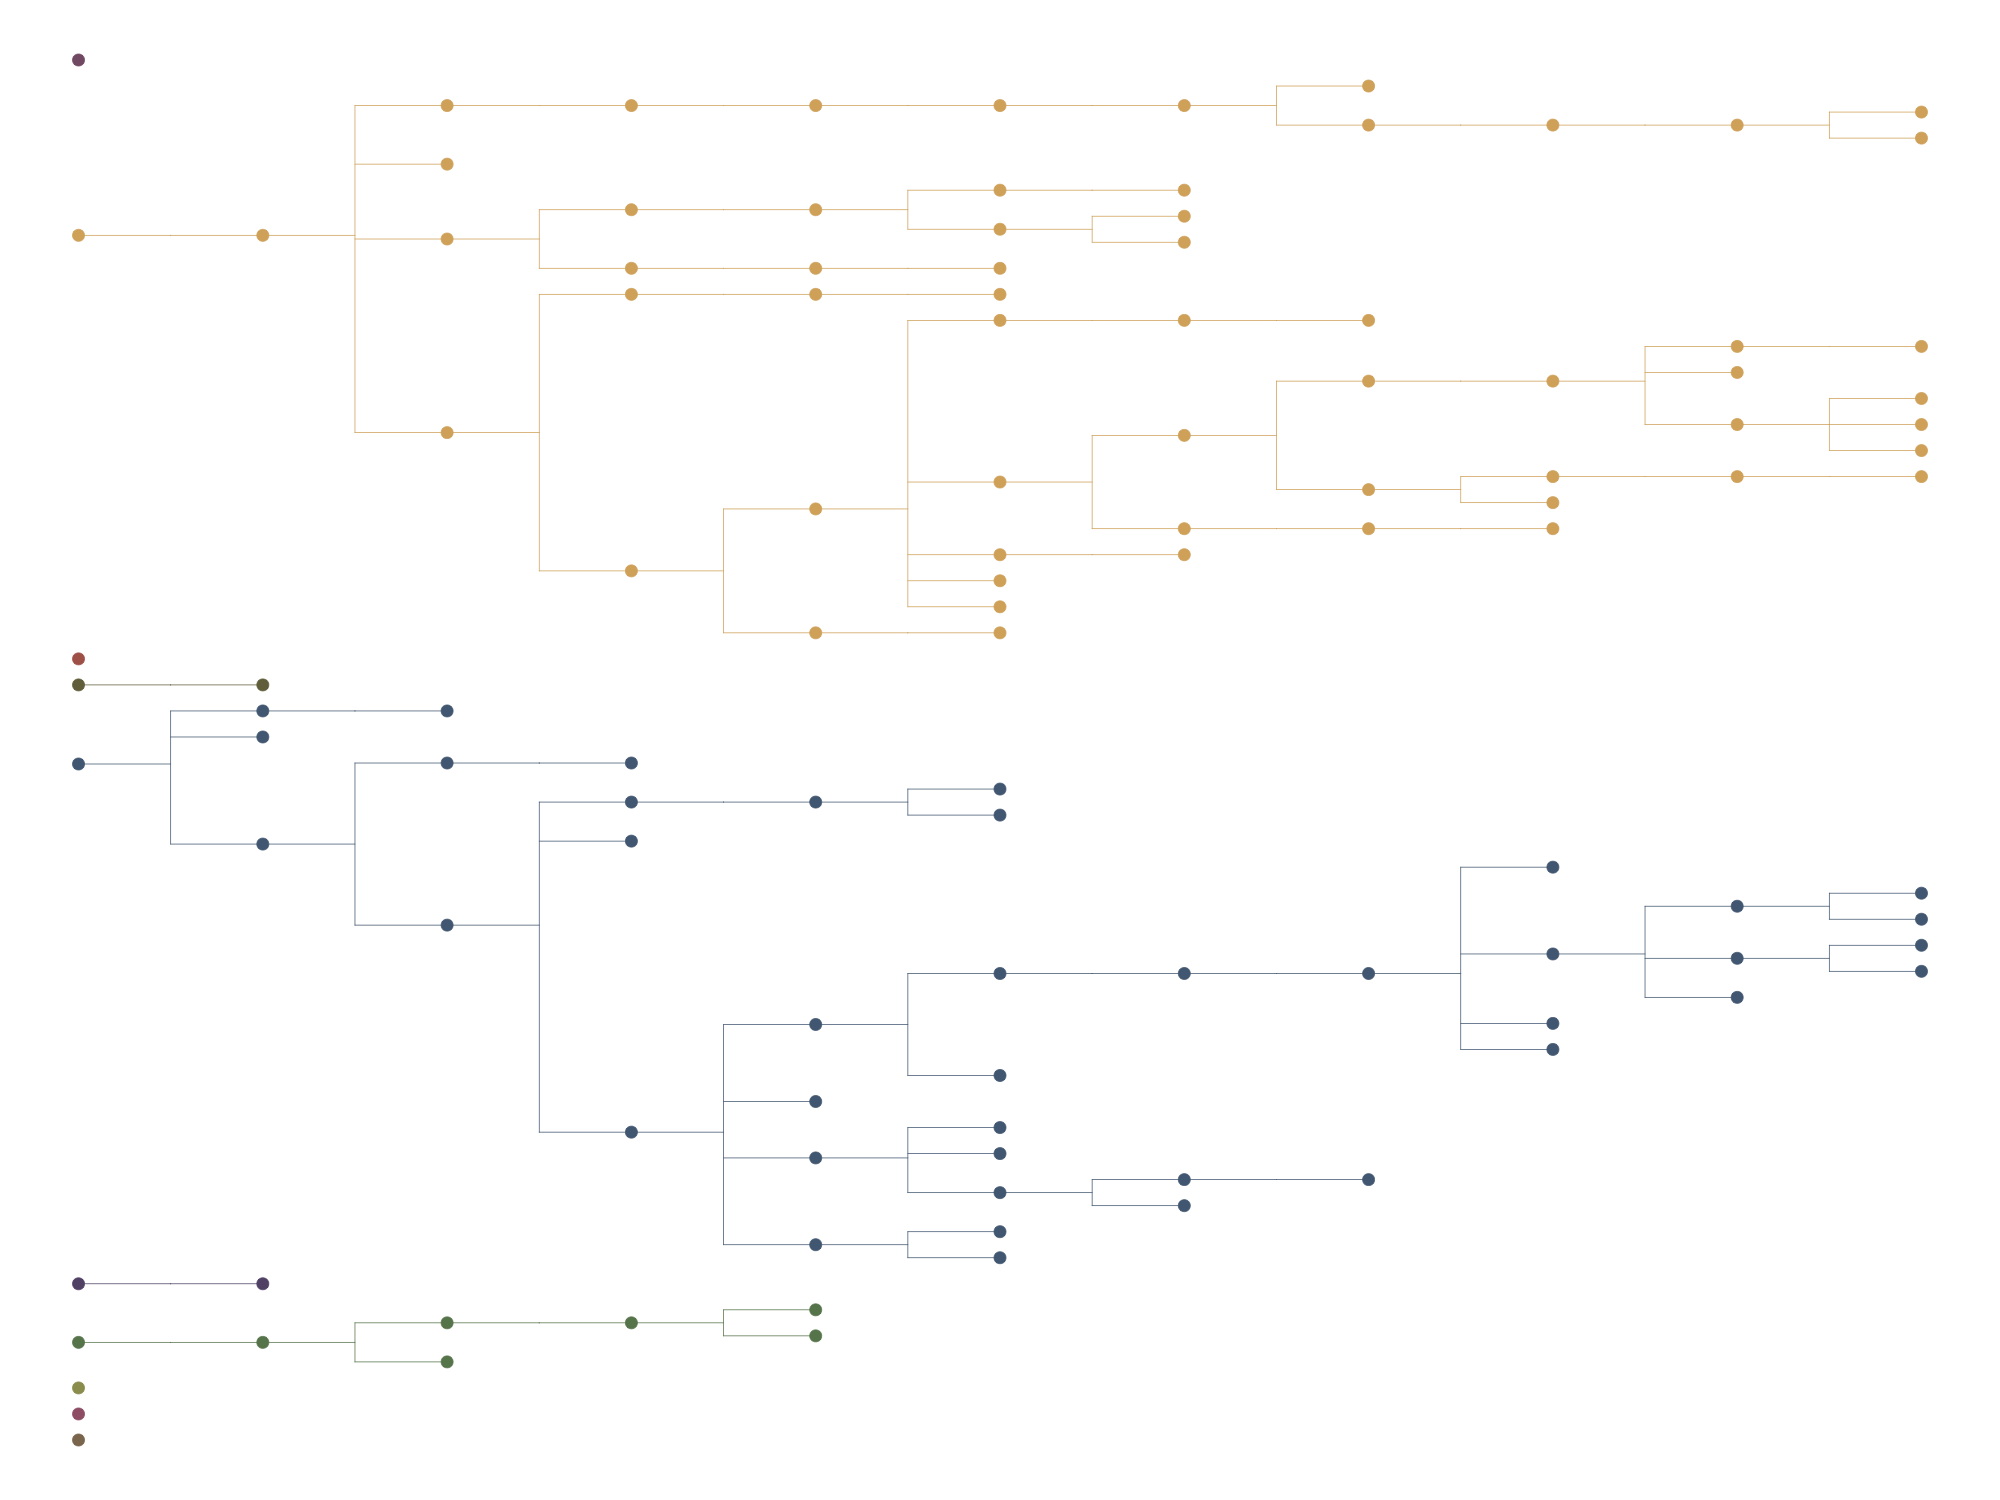
\includegraphics[width=0.8\textwidth,keepaspectratio]{galton_watson.png}
    \caption{Unos arbolitos bien chulos.}
    \label{galton watson}
\end{figure}

%%%%%%%%%%%%%%%%%%%%%%%%%%%%%%%%%%%%%%%%%%%%%%%%%%%%%%%%%
%% No modificar desde esta parte
%%%%%%%%%%%%%%%%%%%%%%%%%%%%%%%%%%%%%%%%%%%%%%%%%%%%%%%%%

\end{document}